
\documentclass[10pt,letterpaper]{article}



% Some useful packages
% math
\usepackage{amsmath}
\usepackage{amsfonts}
\usepackage{algorithm}
\usepackage[noend]{algpseudocode}
\usepackage{amssymb}
% pretty colors
\usepackage{color}
% nicer urls that break at the end of the page
\usepackage{url}
% every document needs images
\usepackage{graphicx}
\usepackage{setspace}
\usepackage{caption}
\usepackage{subcaption}


\newcommand{\e}{\mathbb E}
\newcommand{\R}{\mathbb{R}}
\newcommand\given[1][]{\:#1\vert\:}
\DeclareMathOperator*{\argmin}{arg\,min} % thin space, limits underneath in displays
\DeclareMathOperator*{\argmax}{arg\,max} % thin space, limits underneath in displays
\newcommand{\var}[1]{{\operatorname{\mathit{#1}}}}
\algdef{SE}[SUBALG]{Indent}{EndIndent}{}{\algorithmicend\ }%
\algtext*{Indent}
\algtext*{EndIndent}

\graphicspath{{./figures/}}   % where to look for images

%let's fiddle with the default margins to save some trees
%this makes the odd side margin go to the default of 1inch
\oddsidemargin 0.0in
%sets the textwidth to 6.5, which leaves 1 for the remaining right margin with 8 1/2X11inch paper
\textwidth 6.5in
% less white space, please!
\headheight 0.0in
% shift everything up
\topmargin -0.5in
\footskip .6in
% text should take up all but a 1'' margin
\textheight 9.0in

% Define some shortcuts for things I want to use.
% Use them like, for example:
% \begin{hypothesis}Lettuce causes brain damage.\end{hypothesis}
% Numbering & formatting will happen automatically.
\newtheorem{hypothesis}{Hypothesis}
\newtheorem{task}{Task}
\newtheorem{contribution}{Contribution}


% Shortcuts: allows you to use limited markup when editing/collaborating.
% \comment{This section needs to be rewritten.}
\def\ask#1{\textcolor{red}{\bf $\langle\langle$Question:\ #1$\rangle\rangle$}}
\def\comment#1{\textcolor{red}{\bf $\langle\langle$Comment:\ #1$\rangle\rangle$}}


% This imitates the Wikipedia ``Citation Needed'' text; use it as a temporary
% marker for things you need to cite.
\def\citationneeded{$^{\textcolor{blue}{\text{[citation needed]}}}$ }

% format et al.
\def\etal{\textit{et al.}}
\def\ie{\textit{i.e.}}
\def\eg{\textit{e.g.}}

\title{Attempts to exercise in Reinforcement Learning book Chapter 6}
\author{Mengliao Wang}


\begin{document}

% Generate Title Page
\maketitle


% this dumps the abstract on a front page all by itself.

\section*{Exercise 6.1: }
\label{6.1}

When we add the time stamp to formula 6.5, we would have:

\begin{equation*}
\delta_t = R_{t+1} + \gamma V_t(S_{t+1}) - V_t(S_t)
\end{equation*}

And also we have the equivalence for formula 6.2:
\begin{align*}
V_{t+1}(S_t) &= V_t(S_t) + \alpha\left[R_{t+1} + \gamma V_t(S_{t+1}) - V_t(S_t)\right]\\
&= V_t(S_t) + \alpha\delta_t
\end{align*}

To calculate the difference between $G_t-V(S_t)$ and $\sum_{k=0}^{T-t-1}\gamma^k\delta_{t+k}$, combining the two equations above we have:

\begin{align*}
\Delta &= G_t-V_t(S_t) - \sum_{k=0}^{T-t-1}\gamma^k\delta_{t+k} \\
&= G_t-V_t(S_t) - [R_{t+1} + \gamma V_t(S_{t+1}) - V_t(S_t)] - \gamma[R_{t+2} + \gamma V_{t+1}(S_{t+2}) - V_{t+1}(S_{t+1})] \\
& - \gamma^2[R_{t+3} + \gamma V_{t+2}(S_{t+3}) - V_{t+2}(S_{t+2})] - ... - \gamma^{T-t-1}[R_{T} + \gamma V_{T-1}(S_{T}) - V_{T-1}(S_{T-1})]\\
&= G_t-V_t(S_t) - \sum_{k=0}^{T-t-1}\gamma^kR_{t+k+1} -V_t(S_t) + \gamma[V_{t+1}(S_{t+1}) - V_t(S_{t+1})] \\
& + \gamma^2[V_{t+2}(S_{t+2}) - V_{t+1}(S_{t+2})] + ... + \gamma^{T-t-1}[V_{T-1}(S_{T-1}) - V_{T-2}(S_{T-1})] - \gamma^{T-t}V_{T-1}(S_T)\\
&= \gamma\alpha\delta_{t+1} + \gamma^2\alpha\delta_{t+2} + ... + \gamma^{T-t-1}\alpha\delta_{T-1} - \gamma^{T-t}V_{T-1}(S_T)\\
&= \alpha\sum_{k=1}^{T-t-1}\gamma^{k}\delta_{t+k}
\end{align*}

\section*{Exercise 6.2: }
\label{6.2}

If we move to a new place, and drive from work to the new house will share the same route with the old house, but started to go differently later after the highway. Then for the first few days, Monte Carlo approach will show us the value with a much bigger difference for each state, since the new total expected time at each state is unknown even though we know well enough for the first half of route. Even if the total expected time for each state is only shifted for a few minutes, Monte Carlo is learning the whole return until termination, thus would not take the learnt experience into consideration.

However, for TD method, since it will only update the current state value based on the next state value, at least on the first few days the first half of the route will not see much update. Each state will get much less error on the first half initially.

\section*{Exercise 6.3: }
\label{6.3}

The fact that only $V(A)$ gets updated after the first episode means the first episode ends up terminating on the left side. Since all the states have value initiated to be 0.5 and reward is alway zero unless terminated on the right side, the update $\alpha[R_{t+1} + \gamma V(S_{t+1}) - V(S_t)]$ will always be zero until termination. So no state value will be updated except for the one right before left terminate, which is A. When it terminates, we will see $V(A) = 0.5 + 0.1\times(0 + 0 - 0.5) = 0.45$ as shown in Figure 6.2 left. 


\section*{Exercise 6.4: }
\label{6.4}

If we choose a bigger $\alpha$ for TD approach, it might get worse eventually than the MC approach with a smaller $\alpha$, since we require the $\alpha$ to be small enough for the algorithm to converge. When $\alpha$ increases, both MC and TD approaches will update faster initially, but might not converge to the correct answer. When $\alpha$ decreses, it will update slower at the beginning, but converging to a better answer. So in the longer term, a smaller $\alpha$ will provide a better result for both approaches.


\section*{Exercise 6.6: }
\label{6.6}

The first approach would be using Bellman optimal equation, and we just need to solve the following equations:
\begin{align*}
V(A) &= 0.5\times 0 + 0.5\times V(B)\\
V(B) &= 0.5\times V(A) + 0.5\times V(C)\\
V(C) &= 0.5\times V(B) + 0.5\times V(D)\\
V(D) &= 0.5\times V(C) + 0.5\times V(E)\\
V(E) &= 0.5\times 1 + 0.5\times V(D)\\
\end{align*}

The second approach would be for each state, iterate through all the possible scenarios, and sum up the reward given the probability distribution for each scenarios. For example, for $V(E)$ we would need to sum all the probabilities that it will terminate on the right hand side: $V(E) = \dfrac{1}{2} + \dfrac{1}{2}\times (\dfrac{1}{2})^2+ 2\times \dfrac{1}{2} \times (\dfrac{1}{2})^2 \times (\dfrac{1}{2})^2 + ... = \dfrac{5}{6}$. Obviously we followed the first approach because it is more straight forward to understand and calculate.


\section*{Exercise 6.7: }
\label{6.7}

If we define $\rho_{t:t} = \dfrac{\pi(A_t|S_t)}{b(A_t|S_t)}$, then we have the update rule for TD(0) approach using important sampling:

\begin{equation*}
Q(S_t) = Q(S_t) + \alpha\rho_{t:t}[R_{t+1} + \gamma Q(S_{t+1}, A_{t+1}) - Q(S_t,A_t)]
\end{equation*}


\section*{Exercise 6.8: }
\label{6.8}

Similarly for action values we have the following:
\begin{align*}
G_t - Q(S_t,A_t) &= R_{t+1} + \gamma G_{t+1} - Q(S_t,A_t) + \gamma Q(S_{t+1},A_{t+1})-\gamma Q(S_{t+1},A_{t+1})\\
&= \delta_t + \gamma[G_{t+1} - Q(S_{t+1}, A_{t+1})]\\
&= \delta_t + \gamma\delta_{t+1} + \gamma^2[G_{t+2} - Q(S_{t+2}, A_{t+2})]\\
&= \delta_t + \gamma\delta_{t+1} + ... + \gamma^{T-t-1}\delta_{T-1} + \gamma^{T-t}[G_{T} - Q(S_{T}, A_{T})]\\
&= \sum_{k=t}^{T-1}\gamma^{k-t}\delta_k
\end{align*}

\section*{Exercise 6.9: }
\label{6.9}

\begin{figure}[htp]
\begin{center}
  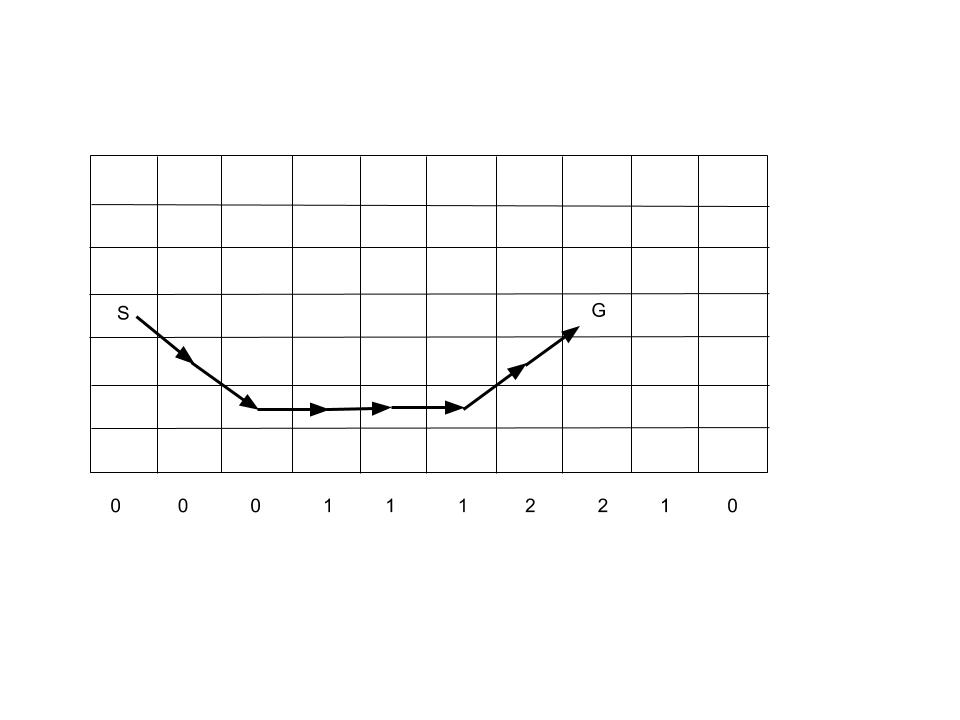
\includegraphics[scale=0.3]{Kings_move_Windy_Gridworld}
\end{center}
  \caption{The solution for windy gridworld task with King's moves}
  \label{fig:king_move}
\end{figure}

The solution for windy gridworld task with King's moves is shown in Figure \ref{fig:king_move}. There won't be any improvement if the ninth action (no movement) is added as it will never be part of the optimal trajectory.


\section*{Exercise 6.10: }
\label{6.10}

The optimal policy is to keep moving right until we reach the destination column. During the path if we are blown away from the center line then we should move in diagonal back towards the center line. After we reach the destination column, we can move vertically towards the destination.


\section*{Exercise 6.11: }
\label{6.11}

Q-learning is considered as an off-policy control method because it samples and learns the value following two different policies. To be more specific, it collects the sample training data based on any soft policy ($\epsilon$-greedy here) which is the behavior policy, and then update the action-value based on the greedy policy which is the target policy, i.e. $\max_aQ(S',a)$.


\section*{Exercise 6.12: }
\label{6.12}

The update equation for Double Expected Sarsa can be written as follows:
\begin{align*}
Q_1(S_t, A_t) &\gets Q_1(S_t, A_t) + \alpha[R_{t+1} + \gamma\sum_a\pi(a|S_{t+1})Q_2(S_{t+1}, a) - Q_1(S_t, A_t))]\\
Q_2(S_t, A_t) &\gets Q_2(S_t, A_t) + \alpha[R_{t+1} + \gamma\sum_a\pi(a|S_{t+1})Q_1(S_{t+1}, a) - Q_2(S_t, A_t))]
\end{align*}

\section*{Exercise 6.13: }
\label{6.13}

It will be natural to implement the Jack Car Rental problem as an afterstate problem. Here instead of defining the state as the car numbers at the end of the day (before we take the actions), we should define it as the car numbers at the beginning of the day (after we take the actions, i.e. move the cars overnight). In this case the action to state transition is explicit and can be calculated with basic algebra. Modeling the problem as afterstate does not only make the implementation easier, but also can speed up the learning speed for state values even though these new states will converge to a different value since the state definition is different. 

\clearpage

\end{document}
